\section{Model Interpretability}
\label{sec:Model_Interpretability}
In the previous section, we have described the design of \sys. In this section, we elaborate on the model interpretability of \sys from the aspects of feature attribution and inter-class distance between traffic types. 

\subsection{Sequence Feature Attribution}
\label{sec:Sequence_Feature_Ranking}
Feature attribution is an important part of model interpretability, which can be divided into global-level attribution and local-level attribution.
The result of the global level attribution is usually the feature ranking of a specific type, while the local level attribution mainly gives the importance of each feature in the prediction of a single sample.

However, existing feature attribution methods are mainly applicable to tabular data and are not designed for network traffic data, which is time series.
If we want these existing feature attribution algorithms to handle the network traffic data, we need to convert the time-series data to tabular data.
A common way to accomplish the above transformation is to reshape the time sequence data.
For example, assume the time sequence data $a$ has a total of $T$ time steps, and each time step is a $d$-dimensional feature vector. We can use \texttt{b = a.reshape(1, $T\times d$)} to reshape the time sequence data $a$ to tabular data $b$ with \textit{NumPy}~\cite{harris2020array}. 
However, this way has two shortages. 
\first This transformation considers features at each time step individually and ignores the relationship between the time sequence data.
\second Current feature ranking methods need a long computation time and have a scalability problem to handle the high-dimensional reshaped data~\cite{zou2016novel}. 

To address the feature attribution of network traffic data, we propose an effective sequence feature attribution method based on \sys.
The interpretability of \sys focuses on the influence of features on fingerprints in terms of time sequence. 
Therefore, \sys provides a new perspective that illustrates the attribution of sequence features.

\begin{figure}[htbp]
	\centering
	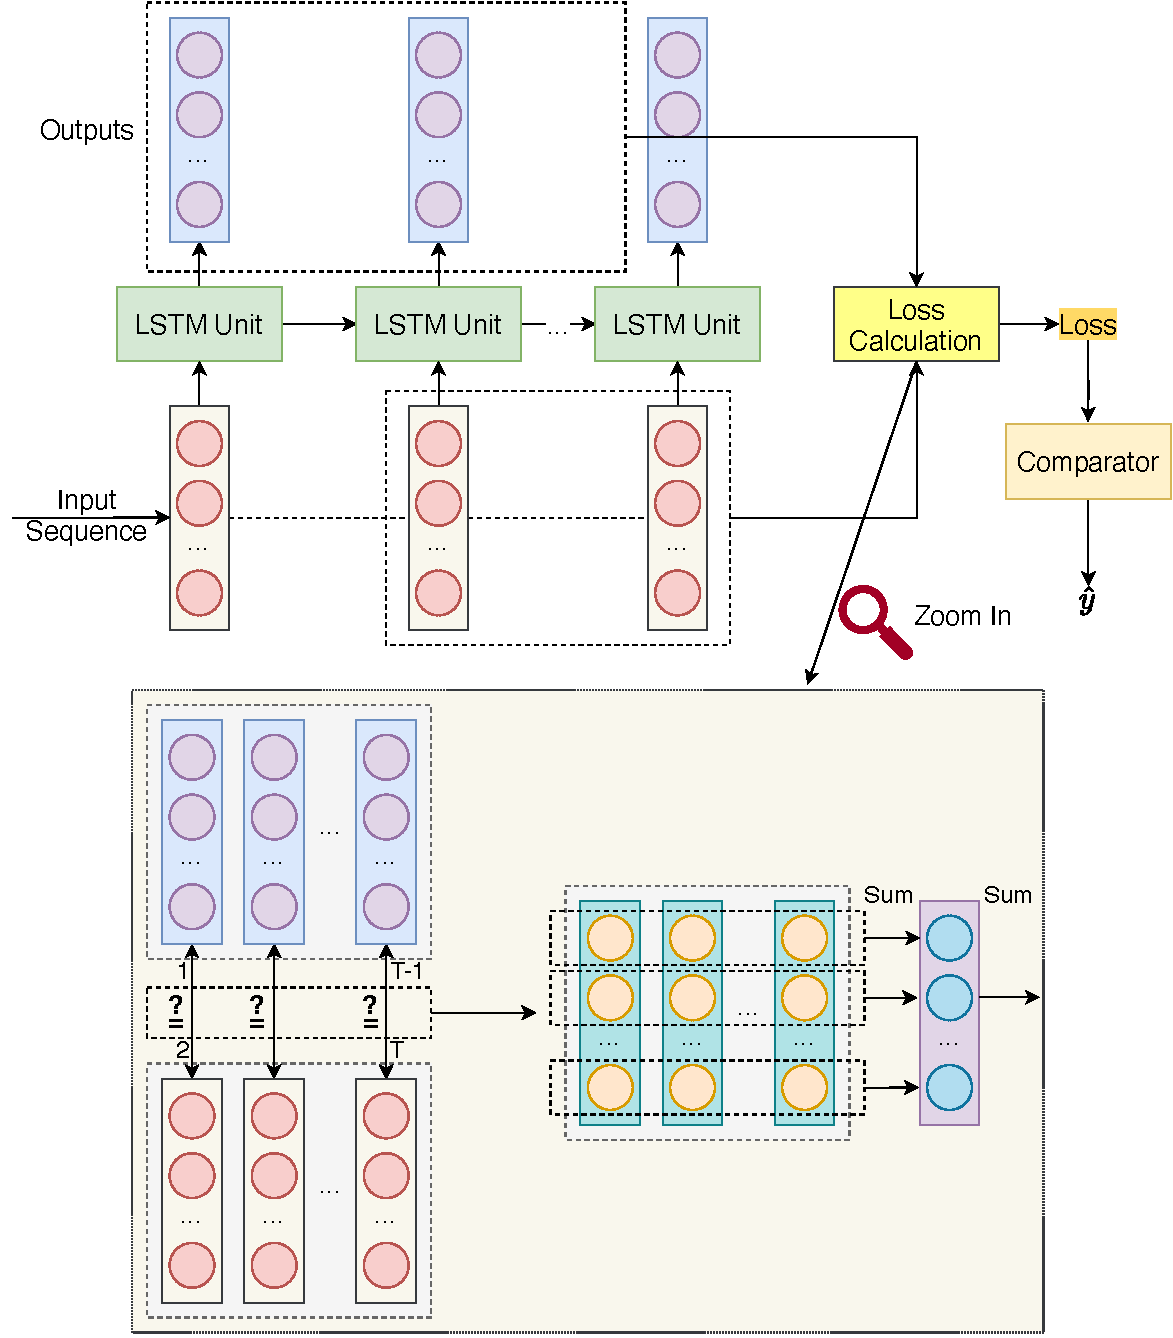
\includegraphics[scale=0.45]{figs/interpretability.pdf}
	\caption{Internal computational process of \sys.}
	\label{fig:interpretability}
\end{figure}

Our feature attribution method stems from the decomposition of the internal computational process of \sys.
Fig.~\ref{fig:interpretability} illustrates the internal computational process of \sys when feeding traffic sequence data.
As mentioned in Section~\ref{sec:Proposed_Traffic_Classification_Method}, each fingerprint module is trained to learn the \emph{fingerprint} (behavioral characteristics) of a specific traffic type and the classification result of the unknown traffic is decided by the fingerprint module with the minimum loss. 
At each time step, the fingerprint module outputs the prediction of the next time step based on the previous input. 
The loss is computed according to Eq.~(\ref{eq:lossfunction}).
Actually, Eq.~(\ref{eq:lossfunction}) is equivalent to first calculating the L2 distance between the output vector and the next input vector at each time step and then summing the distance of each dimension.
Specifically, each dimension of $\mathbf{a_t^{(p)}} - \mathbf{L_{t+1}^{(p)}}$ jointly contributes to the overall loss in Eq.~\eqref{eq:lossfunction}.
Therefore, for a specific traffic type, compared the loss at a certain dimension of the corresponding fingerprint module with losses of other fingerprint modules at the same dimension, if the loss at this dimension is smaller and thus has a larger loss difference, we can say this dimension contributes more to the final prediction and thus ranks higher.
This is the basic idea of our feature attribution method. 
Practically, we feed data of a specific type to all the fingerprint modules in the fingerprint list of \sys. 
We calculate the sum of loss difference in each dimension among fingerprint modules and use it to represent the feature importance.

For formalization, we first define the single-dimensional loss of a sample as
\begin{equation}\label{eq:single-dimensional_loss_sample}
    \mathcal{SL}(\mathbf{x^{(p)}},  \psi_J,  K) = \frac{1}{T-1} \sum_{t=1}^{T-1}\vert \mathbf{a_{J, t}^{(p)}}[K] - \mathbf{L_{t+1}^{(p)}}[K] \vert
\end{equation}
where $\mathcal{SL}(\mathbf{x^{(p)}},  \psi_J,  K)$ represents the $K$-th dimensional loss when feeding sample $\mathbf{x^{(p)}}$ into the $J$-th fingerprint module in the fingerprint list.  
Subsequently, we can calculate the loss difference between fingerprint modules in the $K$-th dimension of a sample $\mathbf{x^{(p)}}$ (abbreviated as feature loss) as follows,
\begin{equation}\label{eq:feature_loss_sample}
\begin{split}
    \mathcal{FL}(\mathbf{x^{(p)}}, K) &= \frac{1}{M}\sum_{J=0}^{M-1} ReLU(\mathcal{SL}(\mathbf{x^{(p)}},  \psi_J,  K) \\
&- \mathcal{SL}(\mathbf{x^{(p)}},  \psi_I,  K))
\end{split}
\end{equation}

The $I$-th fingerprint module only learns the \emph{fingerprint} of traffic type $I$, which is the corresponding type of sample $\mathbf{x^{(p)}}$. 
Consequently, if $I \neq J$, the overall loss $\mathcal{L}_I(\mathbf{x^{(p)}})$ is supposed to be less than $\mathcal{L}_J(\mathbf{x^{(p)}})$, and $K$-th dimension loss $\mathcal{SL}(\mathbf{x^{(p)}},  \psi_I,  K) $ should be less than $\mathcal{SL}(\mathbf{x^{(p)}},  \psi_J,  K) $ correspondingly. 
Therefore, $\mathcal{FL}(\mathbf{x^{(p)}}, K)$ is usually a positive value.  
We use ReLU~\cite{nair2010rectified} to get the non-negative part. 
A larger value indicates that the feature at this dimension contributes more to the difference in the overall loss that the traffic classification relies on. 
Thus we consider the value $\mathcal{FL}(X^I, K)$ as the significance of the feature at the $K$-th dimension of a sample $\mathbf{x^{(p)}}$.

Eq.~\eqref{eq:single-dimensional_loss_sample} and Eq.~\eqref{eq:feature_loss_sample} define the feature importance of a single sample, which offer local interpretability.
For the global interpretability of \sys, we can sum the feature importance of all the samples belonging to traffic type $I$,
\begin{equation}\label{eq:single-dimensional_loss}
\mathcal{SL}(X^I,  \psi_J,  K) = \sum_{\hat{y^{(p)}}=I}\mathcal{SL}(\mathbf{x^{(p)}},  \psi_J,  K) 
\end{equation}
\begin{equation}\label{eq:feature_loss}
\mathcal{FL}(X^I, K) = \sum_{\hat{y^{(p)}}=I} \mathcal{FL}(\mathbf{x^{(p)}}, K)
\end{equation}

\begin{figure}[htbp]
	\centering
	\subfloat[Feature ranking for each traffic type.]{
		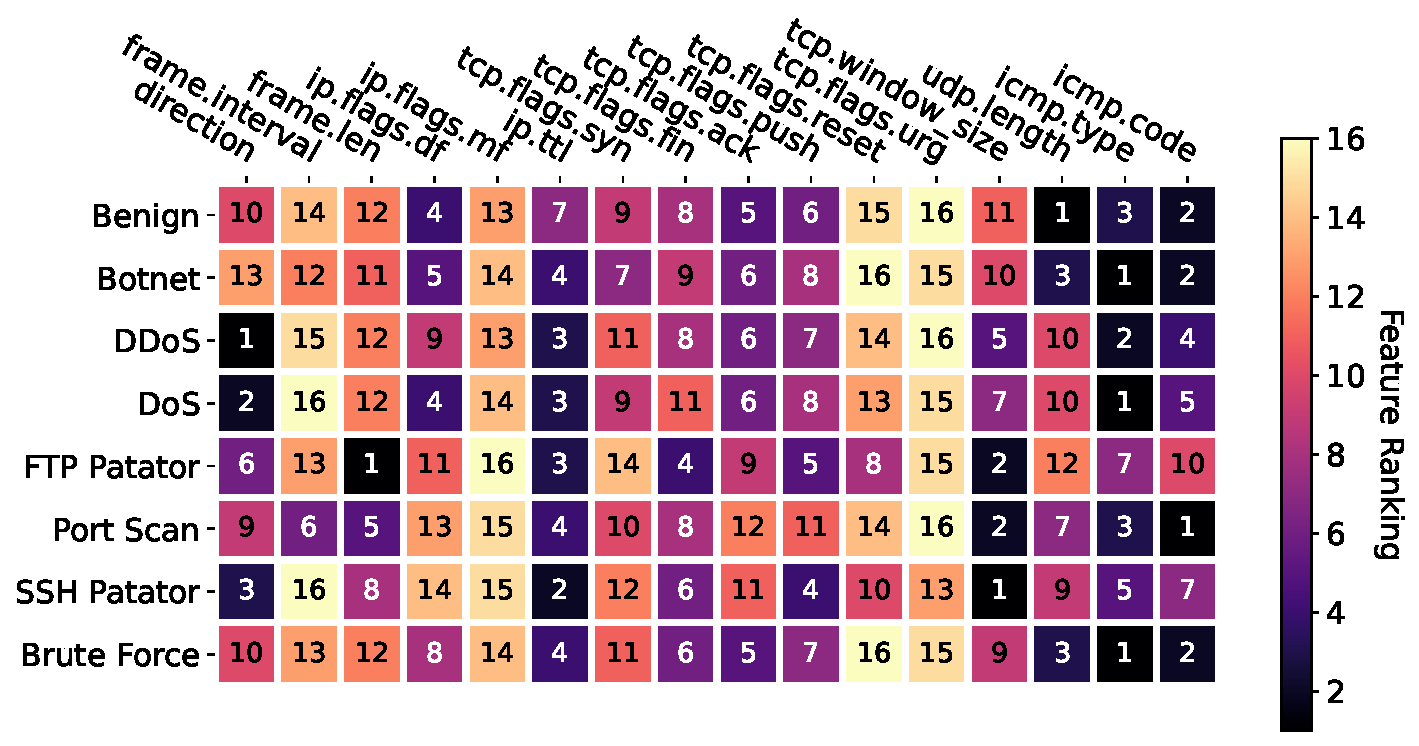
\includegraphics[width=0.95\linewidth]{figs/fingerprint_ids_fingerprint_rank.pdf}
		\label{fig:global_interpret}
	}\\
	\subfloat[Feature importance for classification of traffic samples.]{
		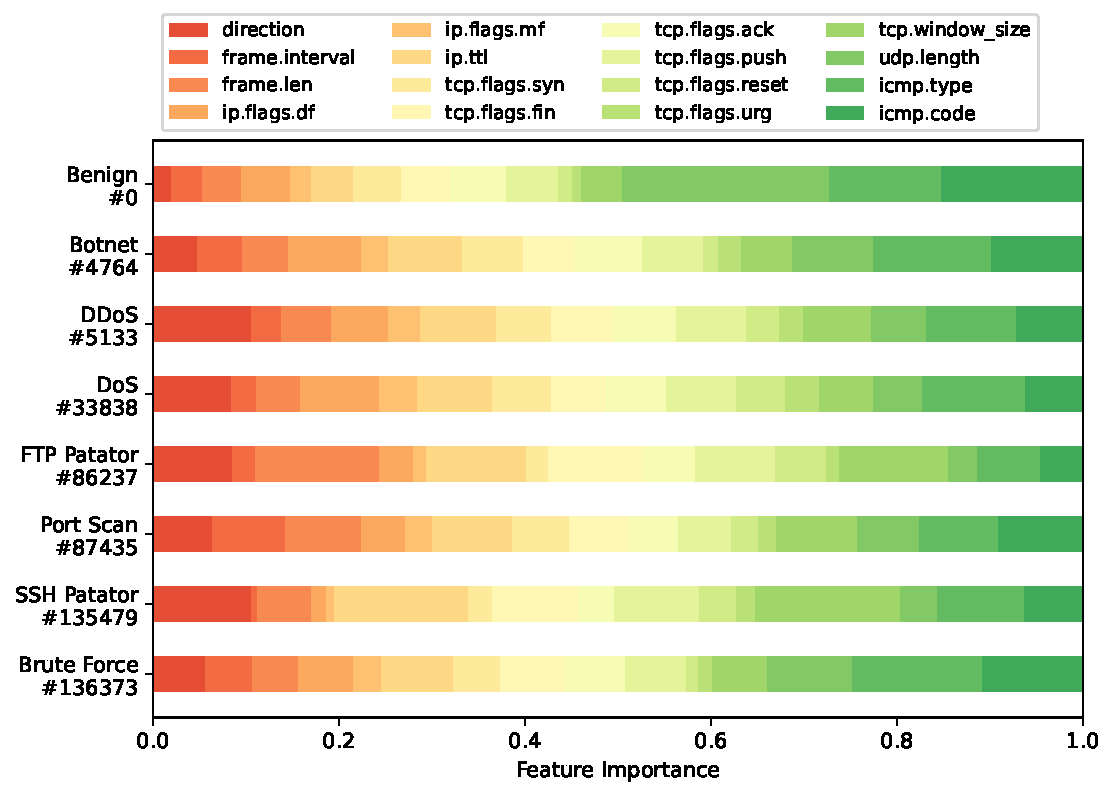
\includegraphics[width=0.95\linewidth]{figs/fingerprint_local_importance.pdf}
		\label{fig:local_interpret}
	}
	\caption{An example of feature attribution results.}
	\label{fig:fea_interpretability}
\end{figure}

Fig.~\ref{fig:fea_interpretability} shows an example of the feature attribution results. 
Fig.~\ref{fig:global_interpret} depicts the feature ranking results for each traffic type.
Each row represents a specific traffic type.
Each column stands for a specific feature.
The numbers inside the square represent the feature ranking (smaller is higher).
These results are interpretable from the perspective of attack principles.
For example, from Fig.~\ref{fig:global_interpret}, we can see that the \emph{direction} is the significant feature for DDoS and DoS.
This is because the communication pattern of these two traffic types is mainly the attacker (the client) sending a flood of packets to the server.
Fig.~\ref{fig:local_interpret} shows the feature importance of samples, illustrating which features contribute more to the classification results.
The numbers on the y-axis are indexes of the selected sample on the dataset. 
It facilitates us to understand how the model comes to the final prediction results.
Take the FTP Patator \#86237 as an example,  we can see that the \emph{frame.len} plays an important role in the classification.
This is mainly because the purpose of the FTP Patator is to keep trying to decipher the password of the FTP server.
Meanwhile, the packet length of the authentication process in FTP is always a fixed value. 

\subsection{Inter-Class Distance between Traffic Types}
\label{sec:inter_class_distance}
According to our design of fingerprint learning, the fingerprint module will output a larger loss if we feed traffic data whose type is not the corresponding type of the fingerprint module.
In other words, the loss is the distance between the input traffic and the expected traffic of the fingerprint module.
In the previous section, we have defined the single-dimensional loss $\mathcal{SL}(X^I,  \psi_J,  K)$ in Eq.(\ref{eq:single-dimensional_loss}), which is the $K$-th dimension of the output loss when feeding traffic data of type $I$ into the $J$-th fingerprint module. 
Based on this, we define the inter-class distance from traffic type $I$ to traffic type $J$ at dimension $K$ as
\begin{equation}\label{equ:traffic_distance}
    \mathcal{DI}(I, J, K) = ReLU(\mathcal{SL}(X^I,  \psi_J,  K) - \mathcal{SL}(X^I,  \psi_I,  K))
\end{equation}
The inter-class distance actually reflects the similarity between traffic types. 
Considering that the distance is always the non-negative value, we use ReLU to extract the non-negative part.
If we take each traffic type as a point and express the distance between the traffic types as an edge between the points, we can draw the distance map on a two-dimensional plane.
Note that in general $\mathcal{DI}(I, J, K) \neq \mathcal{DI}(J, I, K)$ and thus the distance map should be a directed graph. 

\begin{figure}[htbp]
	\centering
	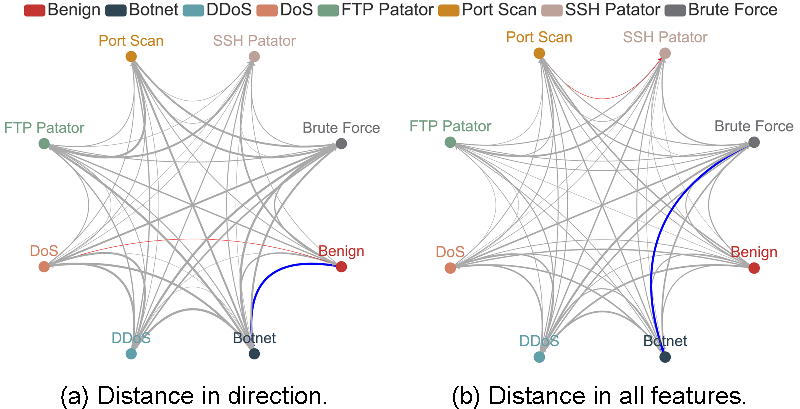
\includegraphics[scale=0.6]{figs/inter_class_distance.pdf}
	\caption{An example of the inter-class distance between traffic types.}
	\label{fig:traffic_distance}
\end{figure}

Fig.~\ref{fig:traffic_distance} shows an example of the inter-class distance between traffic types. 
We use a larger linewidth to represent a smaller inter-class distance. 
In each subfigure, the red and blue lines indicate the largest and smallest inter-class distances, respectively. 
Due to the page limitation, we only present the inter-class distance in the dimension of direction and in all features.
We find the results are rational.
For example, we can see that Port Scan and Brute Force are close in direction. 
This is mainly because the behavior of these two traffic types is similar, \ie attempting to access information about the server by sending massive packets to the target in a short time.
DoS and DDoS are close to each other in all features due to their similar attack behaviors.
Particularly, Benign and Botnet are the closest in direction because they are both bidirectional communication between the client and servers. 
In contrast, DoS and Benign are the farthest in direction as the DoS traffic is usually from clients to the target server while Benign contains bidirectional flows. 
Moreover, we can observe that Botnet and Brute Force are the closest while Port Scan and SSH Patator are the farthest in all features. 
Inspired by this result, we try to group the traffic types with close distances to a new individual type, which may reduce the struggle of the model to distinguish between similar types and improve the classification performance of the model. 
The details of this experiment can be found in Section~\ref{sec:group}.
